\documentclass{article}
\iffalse
This file is protected by Copyright. Please refer to the COPYRIGHT file
distributed with this source distribution.

This file is part of OpenCPI <http://www.opencpi.org>

OpenCPI is free software: you can redistribute it and/or modify it under the
terms of the GNU Lesser General Public License as published by the Free Software
Foundation, either version 3 of the License, or (at your option) any later
version.

OpenCPI is distributed in the hope that it will be useful, but WITHOUT ANY
WARRANTY; without even the implied warranty of MERCHANTABILITY or FITNESS FOR A
PARTICULAR PURPOSE. See the GNU Lesser General Public License for more details.

You should have received a copy of the GNU Lesser General Public License along
with this program. If not, see <http://www.gnu.org/licenses/>.
\fi

\author{} % Force author to be blank
%----------------------------------------------------------------------------------------
% Paper size, orientation and margins
%----------------------------------------------------------------------------------------
\usepackage{geometry}
\geometry{
	letterpaper,			% paper type
	portrait,				% text direction
	left=.75in,				% left margin
	top=.75in,				% top margin
	right=.75in,			% right margin
	bottom=.75in			% bottom margin
 }
%----------------------------------------------------------------------------------------
% Header/Footer
%----------------------------------------------------------------------------------------
\usepackage{fancyhdr} \pagestyle{fancy} % required for fancy headers
\usepackage{multirow}
\usepackage{longtable}
\usepackage{footnote}
\renewcommand{\headrulewidth}{0.5pt}
\renewcommand{\footrulewidth}{0.5pt}
\rhead{\small{ANGRYVIPER Team}}
%----------------------------------------------------------------------------------------
% Appendix packages
%----------------------------------------------------------------------------------------
\usepackage[toc,page]{appendix}
%----------------------------------------------------------------------------------------
% Defined Commands & Renamed Commands
%----------------------------------------------------------------------------------------
\renewcommand{\contentsname}{Table of Contents}
\renewcommand{\listfigurename}{List of Figures}
\renewcommand{\listtablename}{List of Tables}
\newcommand{\todo}[1]{\textcolor{red}{TODO: #1}\PackageWarning{TODO:}{#1}} % To do notes
\newcommand{\code}[1]{\texttt{#1}} % For inline code snippet or command line
%----------------------------------------------------------------------------------------
% Various pacakges
%----------------------------------------------------------------------------------------
\usepackage{hyperref} % for linking urls and lists
\usepackage{graphicx} % for including pictures by file
\usepackage{listings} % for coding language styles
\usepackage{rotating} % for sideways table
\usepackage{pifont}   % for sideways table
\usepackage{pdflscape} % for landscape view
%----------------------------------------------------------------------------------------
% Table packages
%----------------------------------------------------------------------------------------
\usepackage{tabularx} % c=center,l=left,r=right,X=fill
\usepackage{float}
\floatstyle{plaintop}
\usepackage[tableposition=top]{caption}
\newcolumntype{P}[1]{>{\centering\arraybackslash}p{#1}}
\newcolumntype{M}[1]{>{\centering\arraybackslash}m{#1}}
%----------------------------------------------------------------------------------------
% Block Diagram / FSM Drawings
%----------------------------------------------------------------------------------------
\usepackage{tikz}
\usetikzlibrary{shapes,arrows,fit,positioning}
\usetikzlibrary{automata} % used for the fsm
\usetikzlibrary{calc} % For duplicating clients
\usepgfmodule{oo} % To define a client box
%----------------------------------------------------------------------------------------
% Colors Used
%----------------------------------------------------------------------------------------
\usepackage{colortbl}
\definecolor{blue}{rgb}{.7,.8,.9}
\definecolor{ceruleanblue}{rgb}{0.16, 0.32, 0.75}
\definecolor{drkgreen}{rgb}{0,0.6,0}
\definecolor{deepmagenta}{rgb}{0.8, 0.0, 0.8}
\definecolor{cyan}{rgb}{0.0,0.6,0.6}
\definecolor{maroon}{rgb}{0.5,0,0}
%----------------------------------------------------------------------------------------
% Update the docTitle and docVersion per document
%----------------------------------------------------------------------------------------
\def\docTitle{Platform Data Sheet}
\def\docVersion{1.3}
%----------------------------------------------------------------------------------------
\date{Version \docVersion} % Force date to be blank and override date with version
\title{\docTitle}
\lhead{\small{\docTitle}}

\def\comp{alst4}
\edef\ecomp{alst4}
\def\Comp{alst4 Platform}
\graphicspath{ {figures/} }

\begin{document}

\section*{Summary - \Comp}
\begin{tabular}{|c|M{13.5cm}|}
	\hline
	\rowcolor{blue}
	                  &                                                    \\
	\hline
	Name              & \comp                                              \\
	\hline
	Worker Type       & Platform                                           \\
	\hline
	Version           & v\docVersion \\
	\hline
	Release Date      & February 2018 \\
	\hline
	Component Library & ocpi                                        \\
	\hline
	Workers & \comp.hdl                                        \\
	\hline
\end{tabular}

\section*{Functionality}
\begin{flushleft}
The alst4 platform worker provides an interface between a PCIe-connected processor and the Stratix IV FPGA on the Stratix IV Development board. It makes connections over a PCIe bus for OpenCPI control and data planes. It also provides a 200 MHz clock source for the timebase port and a 125 MHz clock source for the control plane.
\end{flushleft}

\section*{Worker Implementation Details}
\begin{flushleft}
	The alst4 platform worker instantiates the pci\_alst4 component from the stratix4 primitive library. The pci\_alst4 component instantiates several components from the pcie\_4243\_hip\_s4gx\_gen2\_x4\_128 library, each of which represent Altera MegaCore-wizard generated IP cores. Figure \ref{fig:blockdiagram} diagrams the intra-worker functionality of the alst4 platform worker, including the functionality of the aforementioned primitive libraries. Note that this diagram is not meant to be an exhaustive diagram of components or their interconnected signals, but a high-level overview of the functionality which includes the worker signals and port connections and how they interact with the instantiated primitives.

	\begin{figure}[h]
		\centering\captionsetup{type=figure}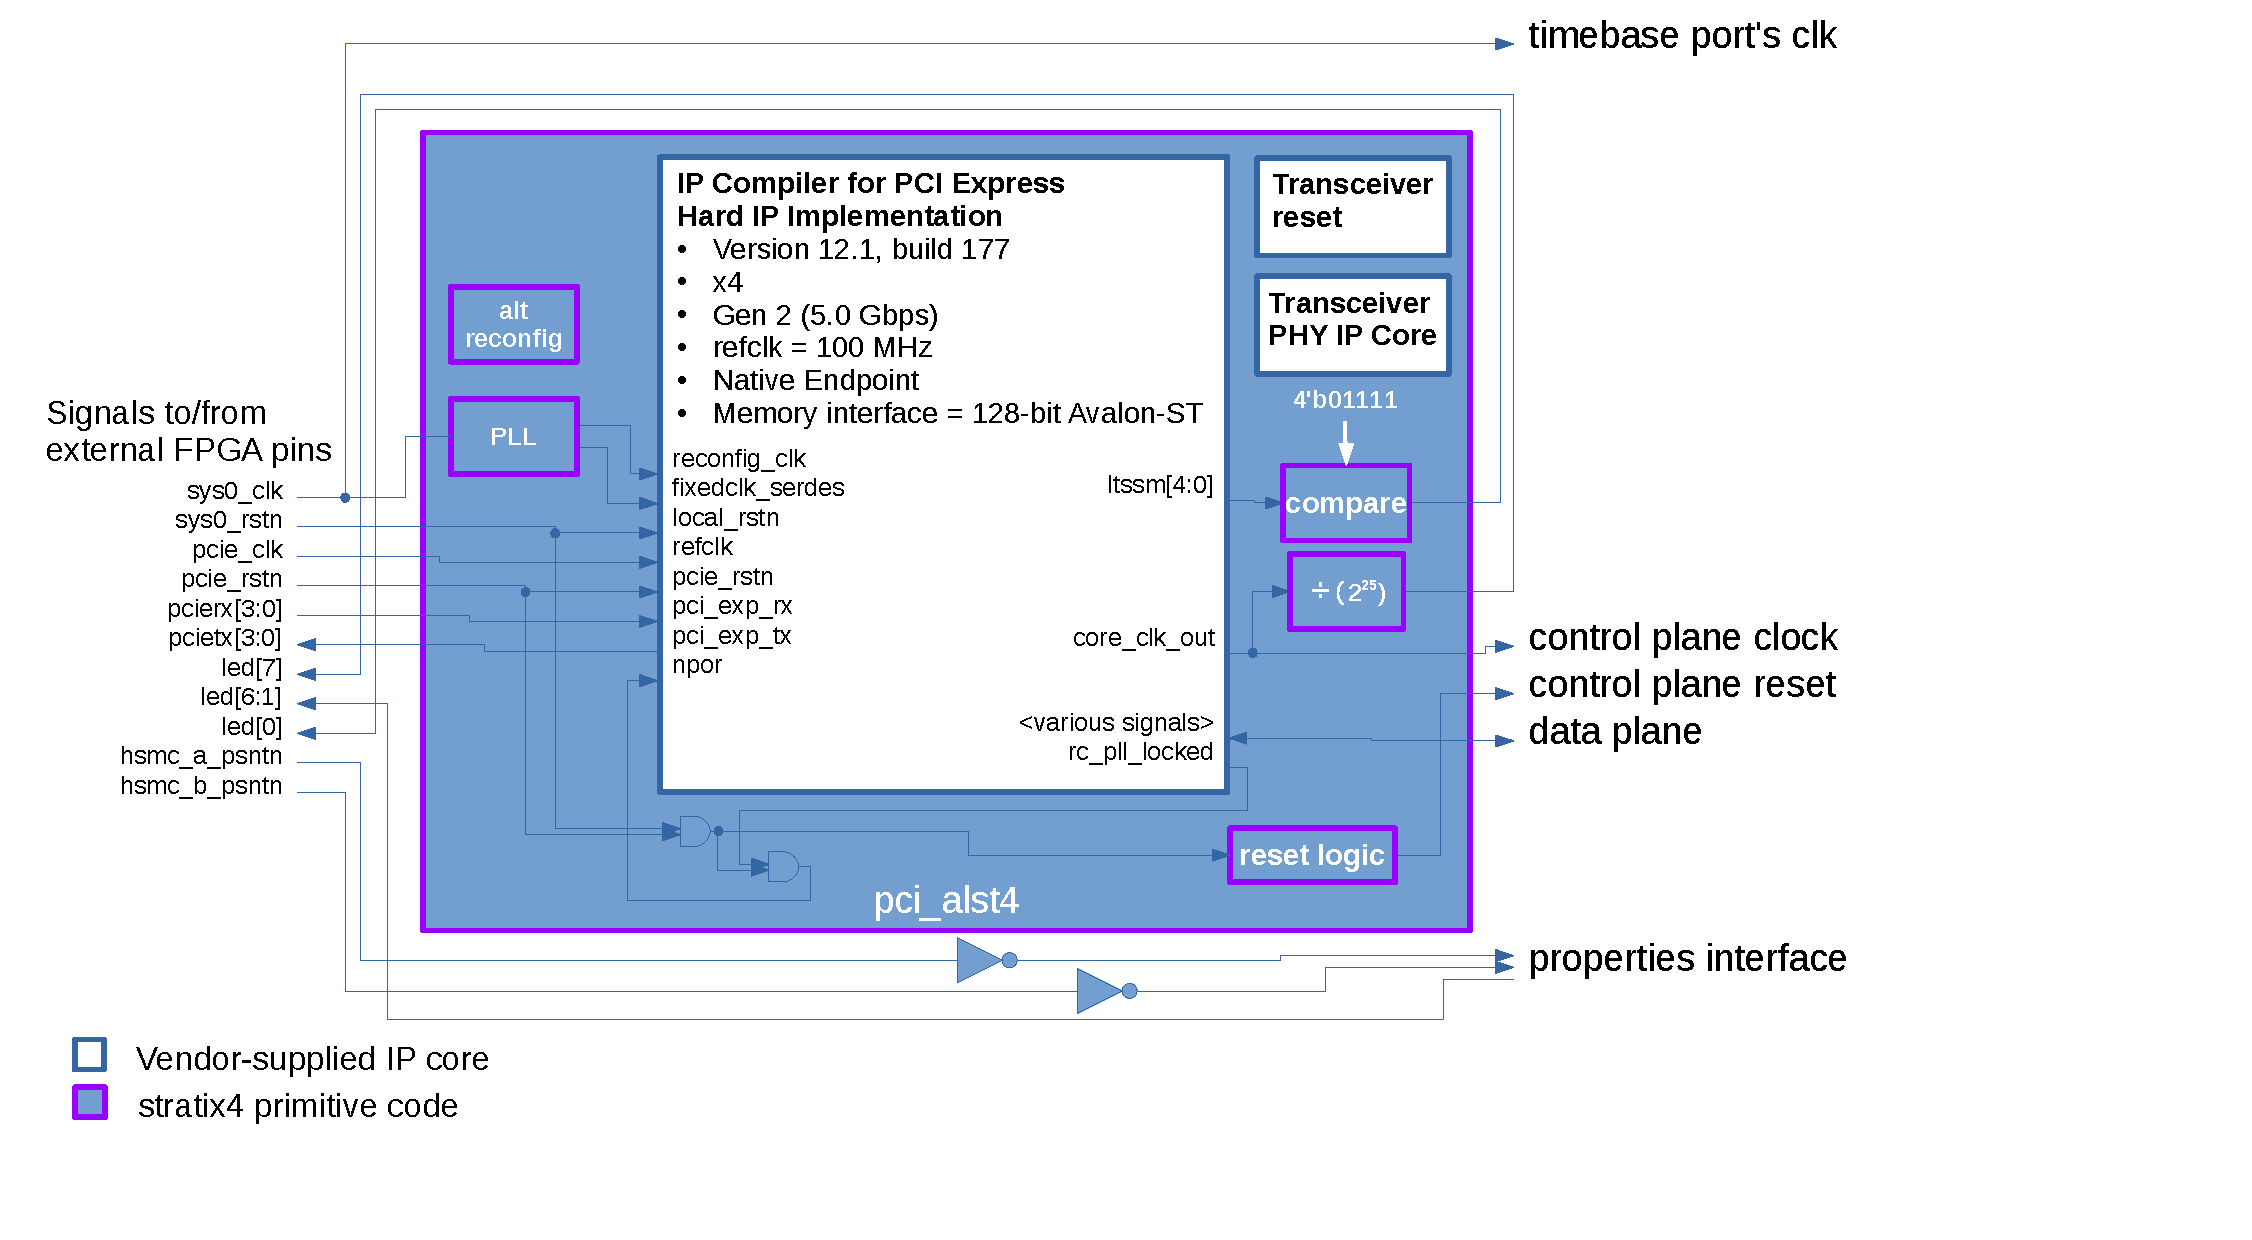
\includegraphics[scale=0.5]{alst4_platform_worker_block_diagram}
		\captionof{figure}{alst4 Functional Diagram}
		\label{fig:blockdiagram}
	\end{figure}
	The pci\_alst4 component instantiates version 12.1 of the PCI Express Hard IP Implementation with Avalon-ST Interface. This implementation is compatible with the PCI Express Card Electromechanical v2.0 specification. The 4-lane Gen2 Implementation is used and a 128-bit Avalon-ST interface is included. Detailed information on the Hard IP Implementation Endpoint with Avalon-ST Interface can be found in the Altera IP Compiler for PCI Express User Guide\footnote{Recommended to start at Figure 4-3 (generic block diagram) and Figure 5-2 (signal I/O diagram)}.
	\subsubsection*{PCIe clocking and reset}
	The Implementation's PCIe clock source is the ref\_clk signal whose intended frequency is 100 MHz. The pcie\_rstn signal is a reset for the PCIe function itself. The reconfig\_clk and fixedclk\_serdes signals allow for transceiver offset cancellation\footnote{See Chapter 13 in the IP Compiler for PCI Express User Guide}. The fixedclk\_serdes signal must be a 125MHz clock which is not generated from the refclk signal\footnote{See page 13-9 in the IP Compiler for PCI Express User Guide}. The local\_rstn is the system-wide asynchronous reset which resets all IP Compiler for PCI Express circuitry not affected by the pcie\_rstn signal. The npor signal is an asynchronous active-low power-on reset. The core\_clk\_out signal produces a clock signal which is fixed at 125 MHz for the given configuration (4 lane, Gen2 Hard IP)\footnote{See Table 7-1 in the IP Compiler for PCI Express User Guide}. The rc\_pll\_locked signal indicates that the SERDES receiver PLL is in locked mode with the reference clock.
	\subsubsection*{PCIe transceiver and Avalon interface}
	Data transmission and reception occurs over the PCIe physical bus via the pci\_exp\_rx and pci\_exp\_tx signal buses. The Avalon-ST data in/out is connected to the data plane via various input/output signals to/from the Implementation.
	\subsubsection*{PCIe link status}
	The ltssm signal bus indicates the Link Training and Status state machine (LTSSM) state, with 0'b01111 indicating L0.\medskip
\end{flushleft}
\pagebreak

\section*{Theory}
Because there are no data processing algorithms implemented in this worker, no corresponding data processing theory is relevant herein.

\section*{Block Diagrams}
\subsection*{Top level}
\makeatletter
\newcommand{\gettikzxy}[3]{%
  \tikz@scan@one@point\pgfutil@firstofone#1\relax
  \edef#2{\the\pgf@x}%
  \edef#3{\the\pgf@y}%
}
\makeatother
\pgfooclass{clientbox}{ % This is the class clientbox
    \method clientbox() { % The clientbox
    }
    \method apply(#1,#2,#3,#4) { % Causes the clientbox to be shown at coordinate (#1,#2) and named #3
        \node[rectangle,draw=white,fill=white] at (#1,#2) (#3) {#4};
    }
}
\pgfoonew \myclient=new clientbox()
\begin{center}
  \begin{tikzpicture}[% List of styles applied to all, to override specify on a case-by-case
      every node/.style={
        align=center,      % use this so that the "\\" for line break works
        minimum size=2cm,  % creates space above and below text in rectangle
        minimum width=4cm
      },
      every edge/.style={draw,thick}
    ]
    \node[rectangle,ultra thick,draw=black,fill=blue](R2){\Comp};
    \node[rectangle,draw=white,fill=white,minimum size=1.0cm](R5)[below= of R2]{timebase};
    \node[rectangle,draw=white,fill=white](placeholder)[above= of R2]{};
    \path[->]
    (R2)edge []  node [] {} (R5)
    (R5)edge []  node [] {} (R2)
    ;
    \gettikzxy{(placeholder)}{\rx}{\ry}
    \myclient.apply(\rx - 40,\ry,C1,\\ metadata);
    \path[<->]($(R2.north) + (-40 pt,0)$) edge [] node [] {} (C1);
    \myclient.apply(-\rx + 40,\ry,C1, ``pcie'' \\ unoc control/data plane );
    \path[<->]($(R2.north) + (40 pt,0)$) edge [] node [] {} (C1);

  \end{tikzpicture}
\end{center}

\subsection*{State Machines}
No state machines exist within the platform worker outside of those within the PCIe MegaCore function. It is not intended for users of MegaCore functions to understand their inner functionality.

\newpage
\section*{Source Dependencies}
\begin{itemize}
	\item
opencpi/hdl/platforms/alst4/alst4.vhd
	\item
opencpi/hdl/primitives/stratix4/altpcie\_reconfig\_4sgx.v
	\item
opencpi/hdl/primitives/stratix4/pci\_alst4.v
	\item
opencpi/hdl/primitives/stratix4/pcie\_hip\_s4gx\_gen2\_x4\_128\_rs\_hip.v
	\item
opencpi/hdl/primitives/stratix4/pcie\_hip\_s4gx\_gen2\_x4\_128\_wrapper.v
	\item
opencpi/hdl/primitives/stratix4/pll1.v
	\item
opencpi/hdl/primitives/pcie\_4243\_hip\_s4gx\_gen2\_x4\_128/altpcie\_hip\_pipen1b.v
	\item
opencpi/hdl/primitives/pcie\_4243\_hip\_s4gx\_gen2\_x4\_128/altpcie\_rs\_serdes.v
	\item
opencpi/hdl/primitives/pcie\_4243\_hip\_s4gx\_gen2\_x4\_128/pcie\_hip\_s4gx\_gen2\_x4\_128\_bb.v
	\item
opencpi/hdl/primitives/pcie\_4243\_hip\_s4gx\_gen2\_x4\_128/pcie\_hip\_s4gx\_gen2\_x4\_128\_core.v
	\item
opencpi/hdl/primitives/pcie\_4243\_hip\_s4gx\_gen2\_x4\_128/pcie\_hip\_s4gx\_gen2\_x4\_128\_serdes.v
	\item
opencpi/hdl/primitives/pcie\_4243\_hip\_s4gx\_gen2\_x4\_128/pcie\_hip\_s4gx\_gen2\_x4\_128.v
	\item
opencpi/hdl/primitives/pcie\_4243\_hip\_s4gx\_gen2\_x4\_128/pciexp\_dcram.v
\end{itemize}

\begin{landscape}
	\section*{Component Spec Properties}
	\begin{scriptsize}
		\begin{tabular}{|p{3cm}|p{1.5cm}|c|c|c|p{1.5cm}|p{1cm}|p{6cm}|}
			\hline
			\rowcolor{blue}
			Name               & Type   & SequenceLength & ArrayDimensions & Accessibility      & Valid Range & Default & Usage                                                                         \\
			\hline
			\verb+platform+    & String & 31             & -               & Parameter & Standard & - & Name of this platform                                                     \\
			\hline
			\verb+sdp_width+   & UChar  & -              & -               & Parameter & Standard & 1 & Width of data plane in DWORDS                                             \\
			\hline
			\verb+UUID+        & ULong  & -              & 16              & Readable           & Standard    & -       & UUID of this platform                                                         \\
			\hline
			\verb+oldtime+     & ULongLong & -           & -               & Padding            & Standard    & -       & N/A                                                                           \\
			\hline
			\verb+romAddr+     & UShort & -              & -               & Writable           & Standard    & -       &                                                                               \\
			\hline
			\verb+romData+     & ULong  & -              & -               & Volatile           & Standard    & -       &                                                                               \\
			\hline
			\verb+nSwitches+   & ULong  & -              & -               & Readable           & Standard    & -       & Number of switches                                                            \\
			\hline
			\verb+nLEDs+       & ULong  & -              & -               & Readable           & Standard    & -       & Number of LEDs                                                                \\
			\hline
			\verb+memories_length+ & ULong & -           & -               & Readable           & Standard    & -       &                                                                               \\
			\hline
			\verb+memories+    & ULong  & -              & 4               & Readable           & Standard    & -       & The memory regions that may be used by \\
  	                     &        &                &                 &                    &             &         & various other elements, which          \\
  	                     &        &                &                 &                    &             &         & inidicates aliasing etc.               \\
                         &        &                &                 &                    &             &         & The values describing each region are: \\
                         &        &                &                 &                    &             &         & Bit 31:28 - External bus/BAR connected \\
                         &        &                &                 &                    &             &         &             to this memory (0 is none) \\
                         &        &                &                 &                    &             &         & Bit 27:14 - Offset in bus/BAR of this  \\
                         &        &                &                 &                    &             &         &             memory (4KB units)         \\
                         &        &                &                 &                    &             &         & Bit  13:0 - Size of this memory (4KB units) \\
                         &        &                &                 &                    &             &         &             units) \\
			\hline
			\verb+dna+         & ULongLong & -           & -               & Readable           & Standard    & -       & DNA (unique chip serial number) of this platform \\
			\hline
			\verb+switches+    & ULong  & -              & -               & Volatile           & Standard    & -       & Current value of any switches in the platform                                 \\
			\hline
			\verb+LEDS+        & ULong  & -              & -               & Writable, Readable & Standard    & -       & Setting of LEDs in the platform, with readback                                \\
			\hline
			\verb+nSlots+      & ULong  & -              & -               & Parameter & Standard & 0 & Number of slots available for cards, which indicates the usable length of the slotCardIsPresent array property. \\
			\hline
			\verb+slotNames+   & String & 32             & -               & Parameter & Standard & "" & A string which is intended to include comma-separated names of the slots available for cards. The inter-comma position of each name corresponds to the same index of the slotCardIsPresent array property. \\
			\hline
			\verb+slotCardIsPresent+ & Bool & -          & 64              & Volatile           & Standard    & -       & An array of booleans, where each index contains an indication whether a card is physically present in the given index's slot. For a description of a given index's slot, see the corresponding comma-separated string contents in the slotName property. Note that only the first min(nSlots,64) of the 64 indices contain pertinent information. \\
			\hline

		\end{tabular}
	\end{scriptsize}
	\section*{Worker Properties}
	\begin{scriptsize}
		\begin{tabular}{|p{1.5cm}|p{2.5cm}|p{1.5cm}|c|c|c|p{2cm}|p{2cm}|p{3cm}|}
			\hline
			\rowcolor{blue}
			Property Type & Name                  & Data Type  & SequenceLength & ArrayDimensions & Accessibility       & Valid Range & Default & Usage                        \\
			\hline
			SpecProperty & \verb+platform+       & String & 31            & -               & Parameter & Standard & alst4 & Name of this platform               \\
			\hline
			SpecProperty & \verb+nSlots+         & ULong  & -             & -               & Parameter & Standard & 2 & Number of slots available for cards, which indicates the usable length of the slotCardIsPresent array property. \\
			\hline
			SpecProperty & \verb+slotNames+      & String & 32            & -               & Parameter & Standard & hsmc\_a,hsmc\_b   & A string which is intended to include comma-separated names of the slots available for cards. The inter-comma position of each name corresponds to the same index of the slotCardIsPresent array property. \\
			\hline
			Property & \verb+pciId+              & UShort & -             & -               & Volatile            & Standard    & -       & Contains PCIe configuration space register contents. See tl\_cfg\_ctl in IP Compiler for PCI Express User Guide. \\
			\hline
			Property & \verb+unocDropCount+      & UChar & -              & -               & Volatile            & Standard    & -       & Invalid packets collected at uNOC terminator \\
			\hline
		\end{tabular}
	\end{scriptsize}

	\section*{Component Ports}
	No ports are implemented for the given component specification.

	\section*{Worker Interfaces}
	\begin{scriptsize}
		\begin{tabular}{|M{2cm}|M{2cm}|M{1.5cm}|M{1.5cm}|M{14.5cm}|}
			\hline
			\rowcolor{blue}
			Type       & Name & Master & Count & Usage                  \\
			\hline
			metadata   & -    & true   & -     & Access to container metadata via the platform worker. All platform workers must provide this port. \\
			\hline
			timebase   & -    & true   & -     & Providing a timebase for the time service. All platform workers must provide this port. \\
			\hline
			unoc       & pcie & true   & -     & This platform worker provides a control/data plane called "pcie". \\
			\hline
		\end{tabular}
	\end{scriptsize}

\end{landscape}
\pagebreak
	\section*{Platform Devices}
	The following is a table which enumerates which device workers are allowed in platform configurations and in assembly containers. The parameter values specified restrict allowed implementations. Note that the worker signals listed are only those who are unconnected on the platform or whose platform signal name differ from the worker signal name. Note that device workers allowed by cards are not included in this list.\\
			\begin{tabular}{|M{3cm}|M{3.5cm}|M{3cm}|M{3cm}|M{3cm}|}
			\hline
			\rowcolor{blue}
			Name                       & Property Name    & Property Value              & Worker Signal & Platform Signal         \\
			\hline
			time\_server               & frequency        & 100*10\textsuperscript{6}   &               &                         \\
			\hline
		\end{tabular}

\section*{Signals}
Note that this signal table does not include signals that may be provided by slots. \\
\begin{tabular}{|c|c|c|c|p{8cm}|}
	\hline
	\rowcolor{blue}
	Name           & Type   & Differential & Width & Description                                          \\
	\hline
	sys0\_clk      & Input  & false        & 1     & 200 MHz clock which is sent to the timebase port as well as supplied to the PCI Express Megacore function for transceiver offset cancellation\footnotemark.    \\
	\hline
	sys0\_rstn     & Input  & false        & 1     & System-wide reset which resets all IP Compiler for PCI Express circuitry not affected by pcie\_rst\_n. This is an asynchronous reset. \\
	\hline
	pcie\_clk      & Input  & false        & 1     & 100 MHz reference clock for the PCI Express IP core. \\
	\hline
	pcie\_rstn    & Input  & false        & 1     & Directly resets all sticky IP Compiler for PCI Express configuration registers. Sticky registers are those registers that fail to reset in L2 low power mode or upon a fundamental rest. This is an asynchronous reset.                                          \\
	\hline
	pcie\_rx       & Input  & false        & 4     & PCIe RX.                                             \\
	\hline
	pcie\_tx       & Output & false        & 4     & PCIe TX.                                             \\
	\hline
	led            & Output & false        & 16    & led[15:0] drive the LEDs labeled '15' through '0', respectively. led[6:1] are driven by the 6:1 indices of the LEDS property. led[7] is driven by the PCIE-generated control plane clock divided by 2\textsuperscript{25} and led[0] is driven by the PCIE link up indicator. A low voltage on these signals illuminates their respective LEDs.\\
	\hline
	hsmc\_a\_psntn          & Input & false & 1    & Connected to the PSNTn signal of the HSMC Port A slot. (Device workers may not ingest the HSMC Port A PSNTn signal). This active-low signal provides FMC LPC mezzanine card presence indication to index 0 of the slotCardIsPresent property.         \\
	\hline
	hsmc\_b\_psntn          & Input & false & 1    & Connected to the PSNTn signal of the HSMC Port B slot. (Device workers may not ingest the HSMC Port B PSNTn signal). This active-low signal provides FMC LPC mezzanine card presence indication to index 0 of the slotCardIsPresent property. \\
	\hline
\end{tabular}
\footnotetext{See Chapter 13 in the IP Compiler for PCI Express User Guide}
\pagebreak
\section*{Slots}
The following table enumerates the available slots for this platform and the signals they include. Note that the signals listed are only those who are unconnected on the platform or whose platform signal name differ from the slot signal name. \\
\begin{longtable}[l]{|c|c|c|c|}
	\hline
	\rowcolor{blue}
	Name           & Type & Slot Signal & Platform Signal  \\
	\hline
	\multirow{2}{*}{HSMC\_ALST4\_A} & \multirow{2}{*}{hsmc\_alst4} & XCVR\_TXp7 & -  \
  \\\cline{3-4}
  & & XCVR\_RXp7 & - \
  \\\cline{3-4}
  & & XCVR\_TXn7 & - \
  \\\cline{3-4}
  & & XCVR\_RXn7 & - \
  \\\cline{3-4}
  & & XCVR\_TXp6 & - \
  \\\cline{3-4}
  & & XCVR\_RXp6 & - \
  \\\cline{3-4}
  & & XCVR\_TXn6 & - \
  \\\cline{3-4}
  & & XCVR\_RXn6 & - \
  \\\cline{3-4}
  & & XCVR\_TXp5 & - \
  \\\cline{3-4}
  & & XCVR\_RXp5 & - \
  \\\cline{3-4}
  & & XCVR\_TXn5 & - \
  \\\cline{3-4}
  & & XCVR\_RXn5 & - \
  \\\cline{3-4}
  & & XCVR\_TXp4 & - \
  \\\cline{3-4}
  & & XCVR\_RXp4 & - \
  \\\cline{3-4}
  & & XCVR\_TXn4 & - \
  \\\cline{3-4}
  & & XCVR\_RXn4 & - \
  \\\cline{3-4}
  & & XCVR\_TXp3 & - \
  \\\cline{3-4}
  & & XCVR\_RXp3 & - \
  \\\cline{3-4}
  & & XCVR\_TXn3 & - \
  \\\cline{3-4}
  & & XCVR\_RXn3 & - \
  \\\cline{3-4}
  & & XCVR\_TXp2 & - \
  \\\cline{3-4}
  & & XCVR\_RXp2 & - \
  \\\cline{3-4}
  & & XCVR\_TXn2 & - \
  \\\cline{3-4}
  & & XCVR\_RXn2 & - \
  \\\cline{3-4}
  & & XCVR\_TXp1 & - \
  \\\cline{3-4}
  & & XCVR\_RXp1 & - \
  \\\cline{3-4}
  & & XCVR\_TXn1 & - \
  \\\cline{3-4}
  & & XCVR\_RXn1 & - \
  \\\cline{3-4}
  & & XCVR\_TXp0 & - \
  \\\cline{3-4}
  & & XCVR\_RXp0 & - \
  \\\cline{3-4}
  & & XCVR\_TXn0 & - \
  \\\cline{3-4}
  & & XCVR\_RXn0 & - \
  \\\cline{3-4}
  & & JTAG\_TCK & - \
  \\\cline{3-4}
  & & JTAG\_TMS & - \
  \\\cline{3-4}
  & & JTAG\_TDO & - \
  \\\cline{3-4}
  & & JTAG\_TDI & - \
  \\\cline{3-4}
  & & PSNTn & - \\
	\hline
	\multirow{2}{*}{HSMC\_ALST4\_B} & \multirow{2}{*}{hsmc\_alst4} & XCVR\_TXp7 & - \
  \\\cline{3-4}
  & & XCVR\_RXp7 & - \
  \\\cline{3-4}
  & & XCVR\_TXn7 & - \
  \\\cline{3-4}
  & & XCVR\_RXn7 & - \
  \\\cline{3-4}
  & & XCVR\_TXp6 & - \
  \\\cline{3-4}
  & & XCVR\_RXp6 & - \
  \\\cline{3-4}
  & & XCVR\_TXn6 & - \
  \\\cline{3-4}
  & & XCVR\_RXn6 & - \
  \\\cline{3-4}
  & & XCVR\_TXp5 & - \
  \\\cline{3-4}
  & & XCVR\_RXp5 & - \
  \\\cline{3-4}
  & & XCVR\_TXn5 & - \
  \\\cline{3-4}
  & & XCVR\_RXn5 & - \
  \\\cline{3-4}
  & & XCVR\_TXp4 & - \
  \\\cline{3-4}
  & & XCVR\_RXp4 & - \
  \\\cline{3-4}
  & & XCVR\_TXn4 & - \
  \\\cline{3-4}
  & & XCVR\_RXn4 & - \
  \\\cline{3-4}
  & & XCVR\_TXp3 & - \
  \\\cline{3-4}
  & & XCVR\_RXp3 & - \
  \\\cline{3-4}
  & & XCVR\_TXn3 & - \
  \\\cline{3-4}
  & & XCVR\_RXn3 & - \
  \\\cline{3-4}
  & & XCVR\_TXp2 & - \
  \\\cline{3-4}
  & & XCVR\_RXp2 & - \
  \\\cline{3-4}
  & & XCVR\_TXn2 & - \
  \\\cline{3-4}
  & & XCVR\_RXn2 & - \
  \\\cline{3-4}
  & & XCVR\_TXp1 & - \
  \\\cline{3-4}
  & & XCVR\_RXp1 & - \
  \\\cline{3-4}
  & & XCVR\_TXn1 & - \
  \\\cline{3-4}
  & & XCVR\_RXn1 & - \
  \\\cline{3-4}
  & & XCVR\_TXp0 & - \
  \\\cline{3-4}
  & & XCVR\_RXp0 & - \
  \\\cline{3-4}
  & & XCVR\_TXn0 & - \
  \\\cline{3-4}
  & & XCVR\_RXn0 & - \
  \\\cline{3-4}
  & & JTAG\_TCK & - \
  \\\cline{3-4}
  & & JTAG\_TMS & - \
  \\\cline{3-4}
  & & JTAG\_TDO & - \
  \\\cline{3-4}
  & & JTAG\_TDI & - \
  \\\cline{3-4}
  & & PSNTn & - \\
	\hline
\end{longtable}
\section*{Platform Configurations}
	\begin{tabular}{|c|c|c|c|}
		\hline
		\rowcolor{blue}
		Name & Platform Configuration Workers & Card & Slot \\
		\hline
		\multirow{2}{*}{base} &\comp & - & - \\ &time\_server & - & - \\
		\hline
		\multirow{5}{*}{alst4\_zipper\_hsmc\_alst4\_port\_a\_rx\_tx} &\comp & - & - \\ &time\_server & - & - \\ &lime\_adc & lime\_zipper\_fmc\_lpc & hsmc\_alst4\_a \\ &lime\_dac & lime\_zipper\_fmc\_lpc & hsmc\_alst4\_a \\ &si5351 & lime\_zipper\_fmc\_lpc & hsmc\_alst4\_a \\ &lime\_rx & lime\_zipper\_fmc\_lpc & hsmc\_alst4\_a \\ &lime\_tx & lime\_zipper\_fmc\_lpc & hsmc\_alst4\_a \\
		\hline
		\multirow{5}{*}{alst4\_zipper\_hsmc\_alst4\_port\_a\_rx} &\comp & - & - \\ &time\_server & - & - \\ &lime\_adc & lime\_zipper\_hsmc\_alst4 & hsmc\_alst4\_a \\  &si5351 & lime\_zipper\_hsmc\_alst4 & hsmc\_alst4\_a \\ &lime\_rx & lime\_zipper\_hsmc\_alst4 & hsmc\_alst4\_a \\
		\hline
		\multirow{5}{*}{alst4\_zipper\_hsmc\_alst4\_port\_a\_tx} &\comp & - & - \\ &time\_server & - & - \\ &lime\_dac & lime\_zipper\_hsmc\_alst4 & hsmc\_alst4\_a \\  &si5351 & lime\_zipper\_hsmc\_alst4 & hsmc\_alst4\_a \\ &lime\_tx & lime\_zipper\_hsmc\_alst4 & hsmc\_alst4\_a \\
		\hline
		\multirow{5}{*}{alst4\_zipper\_hsmc\_alst4\_port\_b\_rx\_tx} &\comp & - & - \\ &time\_server & - & - \\ &lime\_adc & lime\_zipper\_hsmc\_alst4 & hsmc\_alst4\_b \\ &lime\_dac & lime\_zipper\_hsmc\_alst4 & hsmc\_alst4\_b \\ &si5351 & lime\_zipper\_hsmc\_alst4 & hsmc\_alst4\_b \\ &lime\_rx & lime\_zipper\_hsmc\_alst4 & hsmc\_alst4\_b \\ &lime\_tx & lime\_zipper\_hsmc\_alst4 & hsmc\_alst4\_b \\
		\hline
		\multirow{5}{*}{alst4\_zipper\_hsmc\_alst4\_port\_b\_rx} &\comp & - & - \\ &time\_server & - & - \\ &lime\_adc & lime\_zipper\_hsmc\_alst4 & hsmc\_alst4\_b \\  &si5351 & lime\_zipper\_hsmc\_alst4 & hsmc\_alst4\_b \\ &lime\_rx & lime\_zipper\_hsmc\_alst4 & hsmc\_alst4\_b \\
		\hline
		\multirow{5}{*}{alst4\_zipper\_hsmc\_alst4\_port\_b\_tx} &\comp & - & - \\ &time\_server & - & - \\ &lime\_dac & lime\_zipper\_hsmc\_alst4 & hsmc\_alst4\_b \\  &si5351 & lime\_zipper\_hsmc\_alst4 & hsmc\_alst4\_b \\ &lime\_tx & lime\_zipper\_hsmc\_alst4 & hsmc\_alst4\_b \\
		\hline
	\end{tabular}

\section*{Control Timing and Signals}
	There are 3 clock domains present in the alst4 platform worker: 100 MHz, 125 MHz, and 200 MHz. The worker ingests an external-to-the FPGA 100 MHz clock. This clock serves as the clock source for the MegaCore function within the worker. The MegaCore function produces a clock via it's core\_clk\_out pin which is 125 MHz for the x4 Gen2 Avalon-128 implementation\footnote{See Table 7-1 in the IP Compiler for PCI Express User Guide}. This 125 MHz clock is subsequently supplied to the control plane as its clock. The worker also feeds a buffered version of the external-to-the-FPGA 200 MHz clock to the timebase port. The timebase port's PPS inputs and outputs are left unconnected.
\begin{landscape}
\section*{Performance and Resource Utilization}
%-----Filename: alst4_rv.merge.summary
%-----Repo: opencpi.git
%-----Commit ID: a051e972d5ff462242877475684bc639b210da73
%
%Partition Merge Status : Successful - Tue Feb 14 15:59:52 2017
%Quartus Prime Version : 15.1.0 Build 185 10/21/2015 SJ %Standard Edition
%Revision Name : alst4_rv
%Top-level Entity Name : alst4_rv
%Family : Stratix IV
%Logic utilization : N/A
%    Combinational ALUTs : 4,420
%    Memory ALUTs : 0
%    Dedicated logic registers : 3,121
%Total registers : 3121
%Total pins : 1,022
%Total virtual pins : 0
%Total block memory bits : 72,108
%DSP block 18-bit elements : 0
%Total GXB Receiver Channel PCS : 4
%Total GXB Receiver Channel PMA : 4
%Total GXB Transmitter Channel PCS : 4
%Total GXB Transmitter Channel PMA : 4
%Total PLLs : 1
%Total DLLs : 0
In the following Platform Worker Utilization tables, the Worker Build Configuration ``0'' refers to the Platform Worker itself. Named configurations refer to platform configurations (\textit{e.g.} they may include other device workers along with the Platform Worker).\\\\

\input{../../\ecomp/utilization.inc}

\section*{Test and Verification}
\begin{flushleft}
 To be detailed in a future release.
\end{flushleft}
\section*{References}
\begin{flushleft}
	\begin{itemize}
		\item[1)] IP Compiler for PCI Express User Guide, \url{https://www.altera.com/content/dam/altera-www/global/en_US/pdfs/literature/ug/ug_pci_express.pdf} \\

	\end{itemize}
\end{flushleft}
\end{landscape}

\end{document}
